\documentclass[oneside,11pt]{book}

\title{{\sc{spot}} --- Sparco operator toolbox}
\author{Ewout van den Berg \and Michael P. Friedlander}

\usepackage{amsmath}
\usepackage{url}
\usepackage{longtable}
%\usepackage{makeidx}
%\makeindex

\newcommand{\sparco}{Sparco}
\newcommand{\spot}{Spot}
\newcommand{\matlab}{Matlab}
\newcommand{\mlcmd}[1]{\texttt{#1}} % Matlab command

\usepackage{graphicx}
\usepackage{color}
% \definecolor{theshade}{gray}{0.94}
 \definecolor{theframe}{gray}{0.75}
 \definecolor{theblue} {rgb}{0.02,0.04,0.48}
% \definecolor{thered}  {rgb}{0.65,0.04,0.00}
% \definecolor{thegreen}{rgb}{0.06,0.44,0.00}
 \definecolor{thegrey} {gray}{0.5}

 \definecolor{theshade}{gray}{0.98}
 \definecolor{thered}  {rgb}{0.00,0.00,0.00}
 \definecolor{thegreen}{rgb}{0.3,0.3,0.3}

\usepackage{textcomp}
\usepackage{listings}
\lstset{language=matlab,keepspaces,upquote,texcl,
        firstnumber=auto,showstringspaces=false,
        frame=single,gobble=0,
        backgroundcolor=\color{theshade},rulecolor=\color{theframe},
        captionpos=b,
        belowskip=\smallskipamount,
        basewidth={1.25ex},              % Character box base width
        xleftmargin=2.0em,
        xrightmargin=1.0em,
        framexleftmargin=2.0em,
        framexrightmargin=1.0em,
        framesep=0pt,
        breaklines=true,
        basicstyle=\ttfamily,
        keywordstyle=[0]\color{thered},  % Sparco functions
        keywordstyle=[1]\color{theblue}, % Examples
        commentstyle=\color{thegreen},
        keywords=,keywords=[0]{generateProblem,opFoG,opDictionary,opTranspose,opMask,opDCT,opBlockDiag,opBinary,opBernoulli,opBlur,opConvolve1d,opColvolve2d,opColumnRestrict,opRestriction,opCurvelet2d,opDiag,opDirac,opFFT,opFFT2d,opFFT2C,opGaussian,opKron,opPadding,opReal,opWavelet,opWindowedOp,opMatrix,opToMatrix,parseDefaultOpts,getOption,completeOps,dottest,opDifference,parseOptions},
        keywords=[1]{exTV,exSheppLogan}
      }
\lstnewenvironment{codeblock}[1][]{\lstset{#1}}{}

\newcommand{\coderefs}[1]{\noindent $\triangleright$ See further: #1}

\bibliographystyle{plain}

\begin{document}
\maketitle
\tableofcontents

\chapter{Introduction}

The focus of the first version of \sparco{} was to provide a unified
collection of test problems for compressed sensing. Each problem is of
the form
\[
b = MBx_0 + e,\quad \mbox{or}\quad b = Ms + e,
\]
where $b$ is the observed vector, $M$ is a measurement matrix, $s$ is
a signal which can be sparsely represented as the product $Bx_0$,
where $x_0$ is sparse, and $e$ is additive noise. Especially in the
earlier years of compressed sensing (or atomic decomposition), the
sparsity matrix $B$ consisted of a concatenation of sparsity bases
such as the discrete Fourier, cosine, and wavelet transforms. One
salient feature of these transforms is that there exist ways to
evaluate matrix-vector products with these bases, without ever having
to form the underlying matrix explicitly. This leads to fast
multiplication times as well as a high level of scalability in matrix
dimensions. When combining such operators into a compound operator it
is then desirable to preserve these properties. One way to do this is
to write special code for each distinct $B$. This is very time
consuming and a more general framework was set up to implement all
operators. 

After the release of \sparco{} it became increasingly clear that the
operator framework was very useful on its own, which then led to the
development of the \sparco{} operator toolbox (\spot). The aim of the
toolbox is to make operators feel like matrices and allowing many of
the standard methods to be applied to them. The result is a
comprehensive set of operators and methods on operators. Each operator
implements multiplication by itself and by its complex conjugate (or
transpose for real matrices).

%That means that when $A$ and $B$ are some \sparco{} operators, we can
%write
%\begin{codeblock}
%y = A * x;
%z = B'* y;
%\end{codeblock}
%Like with matrices it would also be perfectly fine to write things as
%\begin{codeblock}
%C = B'* A; % Create compound operator
%z = C * x;
%D = [A, B];
%\end{codeblock}

% - Develop sparco, set of test problems for sparse recovery
% - Recognized the need for flexible operators
% - Initially this was done using function handles alone
% - Since then, the flexible set of operators itself became more popular
% - Developed now into full set of operators, still based on function
%   handles to easy of extension, but now wrapped in a Sparco class
% - The aim was to make operators feel like matrices and allowing many
%   of the standard methods to be applied to them.
% - The result (The \sparco{} operator toolbox) is a comprehensive set
%   of operators and methods.


% Element specific operations are slow; and operators such at .*
% cannot be implemented without losing the implicit nature of operators.

%%% Local Variables: 
%%% mode: latex
%%% TeX-master: "manual"
%%% End: 

\chapter{Methods on operators}\label{Sec:SparcoMetaOp} % Operator manipulation

All \sparco{} operators provide routines for multiplying vectors by
itself and its conjugate. The real power of the operator toolbox is
the ease with which basic operators (see Section
\ref{Sec:SparcoOperators}) can be combined into more powerful
operators, which themselves can be combined into yet more powerful
operators. In this section we discuss the type of operations can be
applied to all \sparco{} operators. All operations discussed in this
section are implemented using underlying meta-operators. Pointers to
these operators are given at the end of each section, where
relevant. In the cases where the meta-operators provide more extensive
possibilities, they are described in more detail below the basic use.

We denote by $A$--$D$ arbitrary \sparco{} operators and by $M$ any
matrix. All operator and matrix are assumed to have appropriate
dimensions that can vary line per line. Most operations described in
this section are meaningful only when applied to linear operators; see
\ref{Sec:NonLinearOperators} for more details.

\section{Multiplication}

Multiplication by operators is the most elementary operation in
\sparco. In its simplest form we have operator-vector products such
as:
\begin{codeblock}
y = A * x;
z = B * y;
n = m'* C;  % Evaluated as $n = (C^Hm)^H$
\end{codeblock}
This will evaluate the application of $A$ on $x$, and then $B$ to
$y$. In both cases the result will be an explicit vector of real or
complex numbers. An equivalent approach is to first create a new
operator $C$ representing the product $B\cdot A$, and then apply this
to $x$ to immediately get vector $z$:
\begin{codeblock}
C = B * A;  % Construct compound operator
z = C * x;  % Evaluate $z = BAx$
\end{codeblock}
Although \sparco{} operators are expected to support only
multiplication of vectors, it is possible to write operator-matrix
multiplications. However, it should be kept in mind that this is
implemented as a series of operator-vector multiplications.
\begin{codeblock}
N = C * M;
N = M * C;  % Evaluated as $N = (C^HM^H)^H$
\end{codeblock}
A special case of multiplication is multiplication by
scalars. Generally, this will give a new operator scaled by that
quantity;
\begin{codeblock}
C = 3 * A;  % Construct compound operator $C = 3A$
C = A * 3;
\end{codeblock}
One notable exception is when the corresponding dimension of the
operator is one. In that case we have a valid matrix-vector product
which results in a numeric solution. In other words, matrix-vector
products take precedence over scalar multiplication. In such cases it
is still possible to scale the operator, either by changing the order
(as shown above) or by directly setting the \mlcmd{.scalar} property
of the operator (for more details see Section \ref{Sec:SparcoOpFields}).
Two remaining special cases are multiplication by $\pm 1$, indicated
by the unary plus and minus operations
\begin{codeblock}
C = -A;
B = +A;
\end{codeblock}
This works regardless of the dimensions of the operator. Note that
elementwise multiplication using \mlcmd{.*} is not supported as this
would require the explicit matrix underlying the operator to be known.

In the evaluation and comparison of algorithms it is often useful to
know how many multiplications have been performed using a given
operator. To facilitate these kind of measurements it is possible to
associate a counter variable to each operator. This is discussed in
detail in Section \ref{Sec:SparcoCounters}.

\vspace*{1em}
\coderefs{\mlcmd{opFoG}}

\section{Transposition and conjugation}

As mentioned in the introduction, each \sparco{} operator implements
multiplication by itself and its conjugate. Using \matlab's transpose
operator \mlcmd{'} returns a new operator in which these two modes are
switched.
\begin{codeblock}
B = A';
x = A'* y;
x = B * y; % Identical result as previous line
\end{codeblock}
When using transposes within calculations these new operators are
discarded as soon as the multiplication has been done. Since
transposes in \sparco{} are simple book keeping operations, they are
essentially free; no underlying matrices are actually transposed.
%
The transpose of a complex operator, rather than its conjugate, can be
formed using the \mlcmd{.'} operator. This is implemented as the
elementwise conjugate (see \mlcmd{conj} in Section
\ref{Sec:SparcoConj}) of the conjugate;
\begin{codeblock}
A = C.'; % Transpose of complex operator, $C^T = \overline{(C^H)}$
\end{codeblock}
Note that in this case a single multiplication of a complex vector by
$A$ requires two multiplications by $C^H$ due to the implementation of
the \mlcmd{conj} operation. When applied to a real operator, the
\mlcmd{.'} operation reduces to the standard \mlcmd{'} operation.


\section{Addition and subtraction}

The next elementary operation is the addition and subtraction of
operators. In its simplest for we add two or more operators;
\begin{codeblock}
x = (B + C + D) * y;
A = B + C + D;
x = A * y;           % Equivalent to first statement
\end{codeblock}
When \sparco{} encounters the sum of an operator with a matrix or some
class object that implements the multiplication and size operators, it
will first wrap that entity to a \sparco{} operator using the
\mlcmd{opMatrix} command (see Section \ref{Sec:SparcoOpMatrix}). This
allows us to write
\begin{codeblock}
C = A + M;  % Addition of operator and matrix
C = M + A;  % Addition of matrix and operator
\end{codeblock}
Addition of scalars to an operator is interpreted as an elementwise
addition, just like it is done for matrices. In order to make this
work we first create a new operator of appropriate size, consisting of
only ones (see Section \ref{Sec:SparcoOpOnes}), and premultiply that
with the scalar. The following two statements are therefore equivalent
\begin{codeblock}
A = B + 3;
A = B + 3*opOnes(size(B));
\end{codeblock}
Subtraction is implemented by scalar multiplication combined with
addition.
\begin{codeblock}
A = B - C;
A = B + (-C);
\end{codeblock}
Unfortunately, \sparco{} can only provide a limited amount of
simplification of operators. This means that in the following case, no
simplification is done;
\begin{codeblock}
A = B + 3 - 2; % Not simplified, A = B + 3 - 2;
A = B + C - C; % Not simplified
\end{codeblock}

\coderefs{\mlcmd{opSum}}

\section{Operator information}\label{Sec:SparcoDisp}
\label{Sec:SparcoIsReal}

Before we proceed with more advanced operator manipulations, let us
briefly look at some ways of querying operator information. This kind
of information is useful when developing algorithms and also enable us
to explain how certain operator manipulations work.

The most elementary property of each operator is its size, and it can
be queried using the \mlcmd{size} command. The use of this command is
best illustrated using a number of examples based on a $3\times 6$
operator \mlcmd{A}:
\begin{codeblock}
[m,n] = size(A);    % Gives m = 3, n = 6;
m = size(A,1);      % Gives m = 3;
n = size(A,2);      % Gives n = 6;
o = size(A,3);      % Gives o = 1;
\end{codeblock}
Note that the first two dimensions give the number of rows and columns
respectively. All higher dimensions have size one by definition. To
check if an operator is empty we can use \mlcmd{isempty}:
\begin{codeblock}
if isempty(A)
   error('Operator A cannot be empty');
end
\end{codeblock}
An operator is considered empty if either its number of rows or its
number of columns is zero; a $0\times 6$ operator, albeit of limited
use, is perfectly valid and can be applied to vectors of corresponding
size.

When working interactively from the Matlab command line it is often
more convenient to display the operator by typing its name, or using
the \mlcmd{disp} and \mlcmd{whos} commands. For the following example
we assume that operator $A$ is the operator representation of a
$3\times 6$ matrix (see Section \ref{Sec:SparcoOpMatrix})
\begin{codeblock}
>> A
A is a linear Sparco operator of size 3 x 6
         Matrix(3,6)
>> disp(A)
ans is a linear Sparco operator of size 3 x 6
         Matrix(3,6)
>> whos A
  Name      Size            Bytes  Class       Attributes

  A         3x6              1309  sparcoOp              
\end{codeblock}
The first two commands also provide information about the construction
of the operator:
\begin{codeblock}
>> B = A'*A
B is a linear Sparco operator of size 6 x 6
         (Matrix(6,3))' * Matrix(3,6)
\end{codeblock}

At times, for example during debugging or when using codes not
compatible with \spot{}, it is desirable to have access to the matrix
form underlying an operator. This can be done identically using the
\mlcmd{double}, or \mlcmd{full} commands:
\begin{codeblock}
>> A = opDCT(4);
>> double(A)
ans =
    0.5000    0.5000    0.5000    0.5000
    0.6533    0.2706   -0.2706   -0.6533
    0.5000   -0.5000   -0.5000    0.5000
    0.2706   -0.6533    0.6533   -0.2706
\end{codeblock}
This explicit form is obtained though multiplication by the identity
matrix. As such, it can be quite an expensive operator. When the
number of rows is much smaller than the number of columns it may be
faster to use \mlcmd{double(A')'} instead of \mlcmd{double(A)}.

Finally, the command \mlcmd{isreal} can be used to check if the
operator is real or complex (see Section \ref{Sec:SparcoRealComplex}
for more details on this).  More advanced commands such as
\mlcmd{isfield}, \mlcmd{set}, \mlcmd{get}, and cell indexing will be
discussed in Section \ref{Sec:SparcoImplementation}, which deals with
the implementation of \spot{}.

\section{Dictionaries and arrays}

The original motivation for developing \sparco{} was the concatenation
of operators to form a dictionary. This can now be achieved simply by
writing 
\begin{codeblock}
A = [B,C,M]; % or
A = [B C M];
\end{codeblock}
Note that explicit matrices and classes can be mixed with \sparco{}
operators, provided they are all compatible in size. Like in operator
addition \sparco{} automatically converts these entities to \sparco{}
operators. Vertical concatenation is done likewise by typing
\begin{codeblock}
A = [B;C;M]; % or
A = [B
     C
     M];
\end{codeblock}
With the specification of these two operations, \matlab{} automatically
converts arrays of operators into a vertical concatenation of
dictionaries: 
\begin{codeblock}
A = [B C; C' M]; % or
A = [B   C
     C'  M];     % both represent A = [[B,C];[C',M]];
\end{codeblock}

\coderefs{\mlcmd{opDictionary}, \mlcmd{opStack}}

\section{Block diagonal operators}

Analogous to matrices of operators it is possible to construct block
diagonal operators of operators, using the \mlcmd{diag} and
\mlcmd{blkdiag} commands. Both commands take a list of operators and
matrices to create the desired operator:
\begin{codeblock}
D = diag(A,B,C,M);
D = blkdiag(A,B,C,M);
\end{codeblock}
There is no restriction on the dimension of each operator. This means
that the resulting operator need not necessarily be square:
\begin{center}
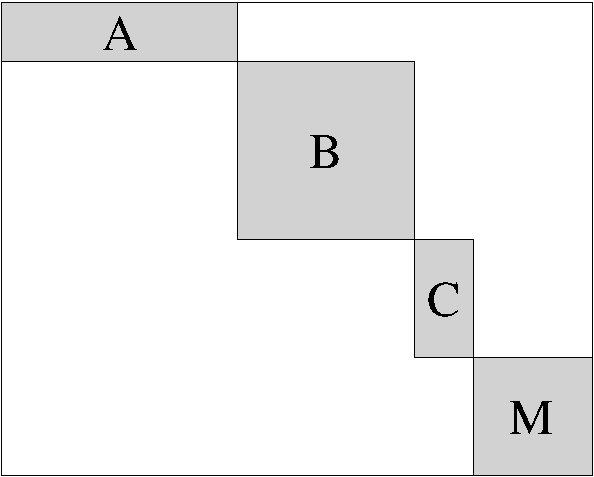
\includegraphics[width=4cm]{./FigSparcoBlockDiag1}
\end{center}
Any matrix or class object that is encountered is automatically
converted into a \spot{} operator. The commands \mlcmd{diag} and
\mlcmd{blkdiag} differ in the way in which explicit vectors are dealt
with in the argument list. Whereas \mlcmd{blkdiag} treats vectors just
like any other matrix, \mlcmd{diag} interprets the vector as the
diagonal entries of a matrix, which is then added as a block. This
behavior is illustrated in the following example
\begin{codeblock}
> D = diag(opDCT(2),ones(2,1)); double(D)
ans =
    0.7071    0.7071         0         0
    0.7071   -0.7071         0         0
         0         0    1.0000         0
         0         0         0    1.0000
> D = blkdiag(opDCT(2),ones(2,1)); double(D)
ans =
    0.7071    0.7071         0
    0.7071   -0.7071         0
         0         0    1.0000
         0         0    1.0000
\end{codeblock}
For more powerful constructions, including horizontal or vertical
overlap of operators the underlying command \mlcmd{opBlockDiag} has to
be called directly.

In section \ref{Sec:SparcoDisp} we illustrated the \mlcmd{isempty}
command on an empty $0\times 6$ operators. Such operators, although
seemingly useless, can come in handy when constructing block-diagonal
operators that require horizontal or vertical padding between certain
blocks.

\paragraph{Advanced interface} The block-diagonal operator can be
invoked in two different ways:
\begin{codeblock}
op = opBlockDiag([weight],op1,...,opn,[overlap]);
op = opBlockDiag([weight],op,[overlap]);
\end{codeblock}
In the first mode, a block-diagonal operator is formed using operators
$1,\ldots,n$, with weights set to
\mlcmd{weight(1)},$\ldots$,\mlcmd{weight(n)}, and a horizontal or
vertical overlap given by parameter \mlcmd{overlap}. Arguments in the
operator list that are not \spot{} operators are automatically
converted using the \mlcmd{opMatrix} command. The sign of the overlap
parameter determines whether overlap should be horizontal or vertical:
\begin{center}
\begin{tabular}{ccc}
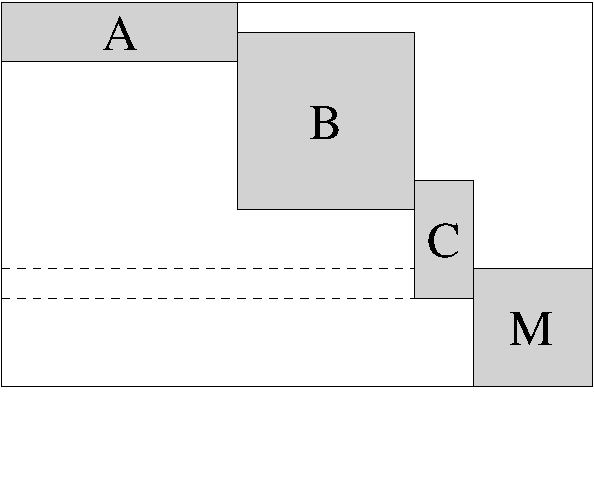
\includegraphics[height=32mm]{./FigSparcoBlockDiag2} & &
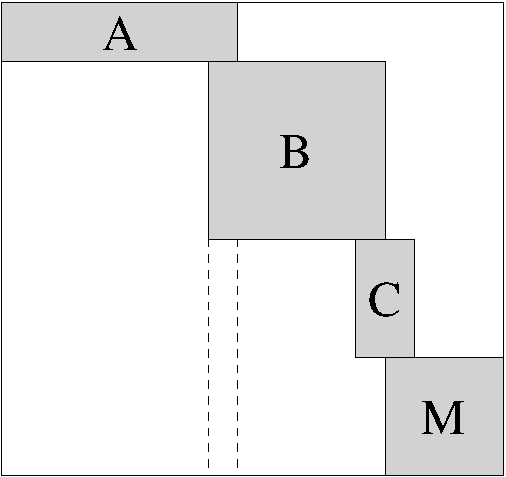
\includegraphics[height=32mm]{./FigSparcoBlockDiag3} \\
Vertical: overlap $>0$ & &
Horizontal: overlap $< 0$
\end{tabular}
\end{center}
The weight and overlap parameters are optional and are set to
\mlcmd{[]}, respectively \mlcmd{0} by default. When the first argument
to \mlcmd{opBlockDiag} is numerical it is interpreted as a weight
parameter, and likewise for the last argument and overlap. Thus,
special care has to be taken when either parameter is omitted while
the first (resp. last) operator is an explicit vector or matrix. This
is best avoided by explicitly specifying the default arguments
whenever ambiguity can arise.

The second mode, with only a single operator specified, can be used to
replicate the given operator. When the vectorized weight parameter,
\mlcmd{weight(:)} is not a scalar its length gives the number of
replications of the operator, each with its corresponding weight. A
scalar weight simply gives the replication count and implies a weight
of one on each operator. Anti-diagonal operators can be obtained by
setting the overlap to twice the dimension of the operator (this also
works in the first mode). An illustration of this with \mlcmd{A} a
$2\times 3$ \sparco{} is given by
\begin{center}
\begin{tabular}{ccc}
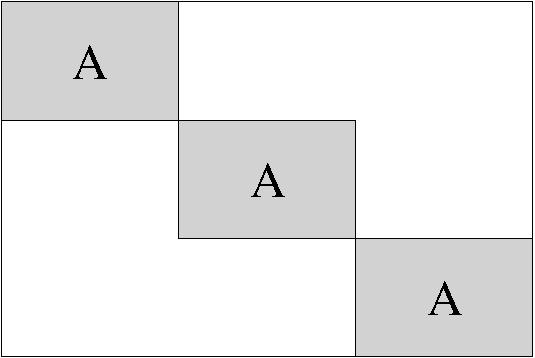
\includegraphics[width=0.3\textwidth]{./FigSparcoBlockDiag4} &
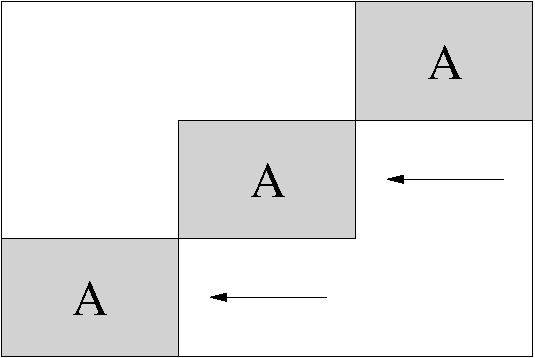
\includegraphics[width=0.3\textwidth]{./FigSparcoBlockDiag5} &
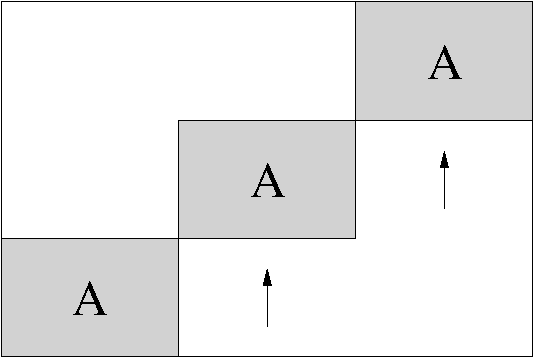
\includegraphics[width=0.3\textwidth]{./FigSparcoBlockDiag6} \\
\mlcmd{opBlockDiag(3,A,0)} &
\mlcmd{opBlockDiag(3,A,-6)} &
\mlcmd{opBlockDiag(3,A,4)}
\end{tabular}
\end{center}


\paragraph{Example}

The block-diagonal operator can be very useful in constructing
windowed Fourier transformations.

\vspace*{1em}
\coderefs{\mlcmd{opBlockDiag}}

\section{Kronecker products}

The \mlcmd{kron} operator allows the creation of Kronecker products
between operators. Unlike \matlab's built-in \mlcmd{kron} function,
the \mlcmd{kron} product in \sparco{} can take an arbitrary number of
arguments. Hence to construct $D = A \otimes B \otimes C$ we can type
\begin{codeblock}
D = kron(A,B,C)
\end{codeblock}
Needless to say, Kronecker products can increase quickly in
computational complexity. Given a set of operators of size $m_i\times
n_i$, $i=1,\ldots,k$, let $m = \prod m_i$, and $n = \prod n_i$. Then,
application of the Kronecker product will require $n / n_i$
multiplications with each operator $i$, and likewise $m / m_i$
products in transpose mode.

\paragraph{Example}
Kronecker products can be useful when operating on high dimensional
data represented in vectorized form. For example, when $x$ represents
a data volume of dimensions $l\times m\times n$.  To create an
operator that applies a one-dimensional Fourier transformation on
vectors along the second dimension, we can simply write
\begin{codeblock}
op = kron(opEye(n),opFFT(m),opEye(l))
\end{codeblock}
Likewise, the block diagonal matrix of three operators $A$, given in
the previous section, could have been created using the Kronecker
product: \mlcmd{kron(opEye(3),A)}. This latter construction was
found to outperform the block diagonal operator consisting of even a
moderate number of identical blocks.

\vspace*{1em}
\coderefs{\mlcmd{opKron}}

\section{Subset assignment and reference}

For certain applications we may be interested only in applying part
of an operator. This can be done by creating new operators that are
restrictions of existing operators. Restriction can be done in terms
of rows, columns, a combination of rows and columns, and in terms of
individual elements of the underlying matrix. Like in matrices, this
is done by indexing using brackets. 
\begin{codeblock}
A = B(3:5,:);     % Extract rows 3-5
A = C(:,4:6);     % Extract columns 4-6
A = D(3:5,4:6);   % Extract rows 3-5 of columns 4-6
\end{codeblock}
The single colon `\mlcmd{:}' indicates that all elements in the given
dimension are selected, and is equivalent to writing the range
\mlcmd{1:end}.
\begin{codeblock}
A = B(3:5,1:end); % Extract rows 3-5
\end{codeblock}
There is no restriction on the ordering of the selected columns and
rows, and it is possible to repeat entries.
\begin{codeblock}
A = B([1,2,2,5,3],end:-1:1); % Extract rows in reverse
\end{codeblock}
Because row and column indexing is implemented by pre- and post
multiplication by selection matrices, the underlying operator is only
applied once for each use of the restricted operator.

In addition to ranges and index lists, it is also possible to use
logicals. In this mode only those entries corresponding to a
\mlcmd{true} value in the logical vector are selected. The length of
the boolean vector must at most be equal to th size of the addressed
dimension. In case it is shorted, additional \mlcmd{false} entries are
added automatically. When using logicals it is not possible to repeat
entries or shuffle them. The following two approaches are logically
equivalent; for performance using logicals may be faster.
\begin{codeblock}
logic = randn(10,1) > 0;
index = find(logic == true);
A = B(logic,:);
A = B(index,:); % Equivalent to previous line
\end{codeblock}
The orientation of the logical or index vector is irrelevant and both
row and column vectors can be used. Dimensions beyond the second one
can be added provided they are either a vector of ones, the empty set
\mlcmd{[]}, or the colon. These additional indices are checked but not
used. Unlike in the matrix case, where \mlcmd{M(1:3,1:4,[])} returns
an empty $3\times 4\times 0$ matrix, the empty set is ignored in the
operator case. It is possible to specify an empty set as the first or
second argument though; this will results in an empty operator of
appropriate size;
\begin{codeblock}
A = B(1:3,[]); % Results in an empty 3-by-0 operator
\end{codeblock}

When indexing with only a single argument the numbers are interpreted
as indices in the vectorized matrix. For a given $m\times n$ matrix,
element $(i,j)$ is accessed by absolute index $(i + (j-1)m)$. In
contrast to indexing by row and column, the result of such operations
will be a vector, rather than an operator. In fact, all required
rows or columns (depending on which one requires fewest applications
of the operator) are first computed and all relevant entries
extracted. When the only parameter is a logical it is first vectorized
and padded with \mlcmd{false} values to the desired length.
A special case is this type of indexing is vectorizing an operator:
\begin{codeblock}
x = B(:); % Vectorized entries of B
y = double(B);
z = y(:); % Same as x
\end{codeblock}
Extracting large numbers of columns or rows from an operator is
computationally expensive since each column or row requires the
multiplication of a vector of the identity matrix by the operator. It
is thus advised to avoid using these operations whenever possible.

\paragraph{Example}

As an illustration of the use of the subset selection we create an
operator that consists of randomly selected rows of a the discrete
Fourier transform. The first step is to construct a Fourier transform
of the desired dimension using the \mlcmd{opFFT} command (see Section
\ref{Sec:SparcoOpFFT}). After that we choose which rows we want to keep
and use subset selection to construct the restricted operator:
\begin{codeblock}
F = opFFT(128);
R = F(rand(128,1)<=0.8,:);
\end{codeblock}
This generates a restricted Fourier operator with approximately 80\%
of all rows selected.

\paragraph{Assignment}

Existing operators can be modified by assigning new values to a subset
of the entries of the underlying matrix representation. For example we
may want to zero out part of some operator $A$:
\begin{codeblock}
A(2,:) = 0;      % Zero out row two
A(:,[3,5]) = 0;  % Zero out columns three and five
\end{codeblock}
These operations are not restricted only to zero values; other
constants can be used as well. With the same ease we can also assign
matrices and other operators to rectangular subsets of existing
operators. In the following two examples we apply this to two $8\times
8$ matrix-based operators $A$ and $B$, and show the resulting operator
format:
\begin{codeblock}
>> A(3:5,[2,4,6]) = randn(3,3)
A is a linear Sparco operator of size 8 x 8
         Embed(Matrix(8,8),Matrix(3,3))

>> B(6:-1:3,4:7) = opDCT(4) 
B is a linear Sparco operator of size 8 x 8
         Embed(Matrix(8,8),DCT(4,4))
\end{codeblock}
Note that in the second example we also flip the rows of the DCT
operator upside down by choosing the row indices from 6 to 3, instead
of the other way around. As long as no destination row or column is
repeated (which is not permitted), and the number of selected rows and
columns matches the size of the operator, any ordering can be used.

The row and column indices may exceed the size of the existing
operator. Such assignments will enlarge the original operator by
logically embedding it into an operator of all zeros prior to
assigning the desired entries with the new operator, matrix or
constant (all are automatically converted to operator form). The cost
of multiplying with the resulting operator depends on whether the
embedded operator overlaps with the original operator or not. Consider
the following example (the \mlcmd{double} command is discussed in
Section \ref{Sec:SparcoDouble})
\begin{codeblock}
>> A = opOnes(2,4); B = 2*opOnes(3,3);
>> A(3:5,3:5) = B;
>> double(A)
ans =
     1     1     1     1     0
     1     1     1     1     0
     0     0     2     2     2
     0     0     2     2     2
     0     0     2     2     2
\end{codeblock}
In this case the operators do not overlap, and multiplication with the
new operator $A$ requires a single application of $B$ and the original
$A$.  Although the command \mlcmd{A(3:5,3:5) = B;} looks like an
update to $A$, what actually happens is that a new operator is
created, which is then linked to variable $A$. The original operator
\mlcmd{A = opOnes(2,4);} still exists but is no longer directly
accessible. Obviously though, it does get used during the
multiplication with the original $A$.

When there is an overlap between the original and embedded operators
the cost of applying the new operator $A$ requires two applications of
the original $A$ and one application of $B$, and likewise for
multiplication by $A^H$.
\begin{codeblock}
>> A = opOnes(2,4); B = 2*opOnes(3,3);
>> A(2:4,3:5) = B;
>> double(A)
ans =
     1     1     1     1     0
     1     1     2     2     2
     0     0     2     2     2
     0     0     2     2     2
\end{codeblock}
In fact, multiplication by the new $A$ takes place in three stages;
the first stage performs multiplication by the original $A$, the
second stage subtracts the influence of the overlap with $B$, and the
third stage adds the result of multiplication by $B$. Note that in
determining overlap \spot{} has to be conservative and assume that the
operators are dense. In the overlapping example above, this means that
assigning a new operator to \mlcmd{A(3:4,1:2)} does count as and
overlap even though this neither overlaps with the original $A$, nor
with $B$. When an operator consists of a number of non-overlapping
blocks it is therefore recommended to add the operators in such an
order that as few conservative decisions have to be
made. Alternatively, a new meta-operator could be created to
accommodate such constructions.

A special situation arises when assigning the empty set \mlcmd{[]} to
a subset of rows or columns. Doing so causes the given rows or columns
to be deleted from the operator. Continuing with the above $4\times 5$
overlapped operator $A$, we have
\begin{codeblock}
>> A(:,[1,3]) = [];
>> double(A)
ans =
     1     1     0
     1     2     2
     0     2     2
     0     2     2
>> A([2,3],:) = [];
>> double(A);
ans =
     1     1     0
     0     2     2
\end{codeblock}
While the above example uses the colon (\mlcmd{:}) it is also possible
to use \mlcmd{1:end}, \mlcmd{end:-1:1}, or any (logical) set of
indices that covers all rows or columns. Cutting rows or columns is
implemented by respectively pre- and post multiplying by a selection
matrix. This means that multiplication by the resulting operator still
requires application of the full original operator whether or not the
relevant rows or columns are needed.

Assignment using absolute index numbers is not supported in the
current version of \spot{}. For the above $2\times 3$ operator $A$,
the command \mlcmd{A(5) = 3;} will thus generate an error.


% Alternatively we can cut those rows out
% F(rand(128,1)>0.8,:) = [];


% Subset assignment and reference, and use of `end'
% -----------------------------------------------------------
% Setting subsets we need to multiply, subtract existing subset and
% then add new subset, in terms of performance this not ideal
% When operating on subsets, the number of operations are tried to be
% kept to a minimum by rectangular grids, in case absolute element
% numbers (row + col*number of rows) this may be very costly.

\vspace*{1em}
\coderefs{\mlcmd{opRestriction}}


\section{Elementwise operations} \label{Sec:SparcoConj}
                                      \label{Sec:SparcoDouble}

There are a number of operations that, just like multiplication by
scalars, affect all individual entries of matrix underlying the
operator. For complex operators \spot{} provides the commands
\mlcmd{real}, \mlcmd{imag}, and \mlcmd{conj}. The first command
discards the imaginary parts of the operator and results in a real
operator, while the second command keeps only the imaginary part of
the operator (this results in a real number operator). The
\mlcmd{conj} command replaces each element by its complex
conjugate. When applied to a real operator \mlcmd{real} and
\mlcmd{conj} do nothing, while \mlcmd{image} returns a new zero
operator (all underlying operators are discarded). Due to 
self-awareness, applying conjugation to a conjugated operator cancels
the conjugation.

\begin{codeblock}
F = opMatrix(2 + 3i);
a = real(F);          % a = opMatrix(2)
b = imag(F);          % b = opMatrix(3)
c = conj(F);          % c = opMatrix(2 - 3i)
\end{codeblock}

Application of \mlcmd{real}, \mlcmd{imag}, or \mlcmd{conj} leads to
the creation of a new operator. Provided the new operator is not the
zero operator, multiplication is implemented by distinguishing between
real, imaginary, and complex vectors. In the first two cases a single
application of the underlying operator suffices. For complex vectors
we need to apply the underlying operator to both the real and
imaginary parts of the vector and combine the results according to the
desired operation, thus requiring two operations per multiplication.

\vspace*{1em}
\coderefs{\mlcmd{opReal}, \mlcmd{opImag}, \mlcmd{opConj}, \mlcmd{isreal}}

\section{Power, inverse, and backslash operations}

The operations discussed in this section are provided for convenience,
but they should be used with care to avoid prohibitively slow or
inaccurate operators. With that said, the power operator \mlcmd{\^} or
\mlcmd{mpower} takes a square operator and raises it to a given
integer power. The following code illustrates the semantics of the
power operator, when applied to a square operator $A$
\begin{codeblock}
B = A^3            % A*A*A
B = mpower(A,3)    % A*A*A
B = mpower(A,0)    % A\texttt{\^}0 = opOnes(size(A))
B = mpower(A,-3)   % A\texttt{\^}-3 = inv(mpower(A,3))\hspace*{-10pt}}
\end{codeblock}
The \mlcmd{inv} command constructs an operator that represents the
inverse of the given square operator, and is implemented using the
\mlcmd{opInverse} operator. Multiplication by this operator is done by
solving a least-squares system using LSQR \cite{PaigSaun:1982}. Hence,
$y$ in the following code
\begin{codeblock}
B = opInverse(A);
x = B * b;
\end{codeblock}
is computed by solving
\begin{equation}\label{Eq:LSQR}
\mathop{\mbox{minimize}}_{x}\quad \Vert Ax - b\Vert_2,
\end{equation}
with additional regularization to obtain the least two-norm solution
$x$ in case the system is underdetermined. Because the least-squares
problem is not restricted to square matrices, \mlcmd{opInverse} can
also be applied on rectangular operators to give the
pseudo-inverse. When $A$ is an $m\times n$, it is obvious from the
above problem that $B$ must be an $n\times m$ operator.  Due to the
need to to solve a least-squares problem with each matrix-vector
product, the use of the inverse operators is computationally
expensive.

The \mlcmd{opPower} command with a negative exponent corresponds to
applying the inverse to the operator raised to the magnitude of the
exponent. In other words, writing $A^{-2}$ is implemented as
$(A^2)^{-1}$. When the inverse of an inverted operator (or one with
negative power) is taken, the inverses cancel and the result will be
the original operator, regardless of any possible singularity.

Finally, the backslash operator \mlcmd{$\setminus$} can be used to
represent the least-squares problem \eqref{Eq:LSQR}. With this
operator, the above code block can be written without introducing $B$:
\begin{codeblock}
x = A \ b;
\end{codeblock}
When $A$ is underdetermined the resulting $x$ may not be the same as
\mlcmd{x = double(A) $\setminus$ b}, because the latter does not necessarily
give the least two-norm solution $x$.
In compliance with \matlab's \mlcmd{mrdivide} operator, or \mlcmd{/}
for short, \spot{} implements the matrix division $A/B$ as $(B^H \setminus
A^H)^H$. Obviously $A/3$ is implemented as $(1/3)A$.


\vspace*{1em}
\coderefs{\mlcmd{opInverse}, \mlcmd{opPower}}

\section{Solving systems of linear equations}

Matlab provides a number of routines for solving systems of linear
equations that either take a matrix or a function handle. Wrappers to
these function that take \spot{} operators are implemented for the
following functions:
\begin{longtable}{|p{2.8cm}p{9.0cm}|}
\hline
\mlcmd{bicg}     & Biconjugate gradients method \\
\mlcmd{bicgstab} & Biconjugate gradients stabilized method \\
\mlcmd{cgs}      & Conjugate gradients squared method \\
\mlcmd{gmres}    & Generalized minimum residual method \\
\mlcmd{lsqr}     & Least-squares method \\
\mlcmd{minres}   & Minimum residual method \\
\mlcmd{pcg}      & Preconditioned conjugate gradients method \\
\mlcmd{qmr}      & Quasi-minimal residual method \\
\mlcmd{symmlq}   & Symmetric LQ method \\
\hline
\end{longtable}


\section{Application to non-linear operators}\label{Sec:NonLinearOperators}

In some situations it may be desired to create nonlinear
operators. For example, when the output of a certain series of
operations on complex input is known to be real it may be desired to
have an operator that discards the imaginary part of its input. While
\spot{} permits the construction of such operators (see the
\mlcmd{.linear} field in Section \ref{Sec:SparcoOpFieldLinear}),
utmost care has to be taken when using them in combination with meta
operators. Because there are no sanity checks in the implementation of
the meta operators, application to nonlinear operators is not
guaranteed to be meaningful; this is something the user should
decide.

%%% Local Variables: 
%%% mode: latex
%%% TeX-master: "manual"
%%% End: 

\chapter{Basic operators}\label{Sec:SparcoOperators}

In this chapter we discuss the atomic operators that can be combined
to more complicated operators using the methods described in the
previous section.

\section{Elementary operators}\label{Sec:SparcoOpOnes}

The most elementary operators are created by the following commands:
\vspace*{.5em}

\noindent
\begin{tabular}{|p{2.4cm}p{9.4cm}|}
\hline
\mlcmd{opEye(m,n)}
& Creates an $m\times n$ operator with ones on the diagonal. When
  omitted, $n$ is set to $m$. Calling \mlcmd{opEye} without arguments
  creates an operator representing the scalar 1.\\
%
\mlcmd{opDirac(n)}
& Same as \mlcmd{opEye(n,n)}. When omitted, $n$ is set to 1. \\ 
%
\mlcmd{opZeros(m,n)}
& This creates an identically zero $m\times n$ operator. When omitted,
  $n$ is set to $m$. Calling \mlcmd{opZeros} without arguments creates
  an operator representing the scalar 0.\\
\mlcmd{opOnes(m,n)}
& This creates an $m\times n$ operator consisting of all ones. When
  omitted, $n$ is set to $m$. Calling \mlcmd{opOnes} without
  arguments creates an operator representing the scalar 1. \\
\mlcmd{opDiag(d)}
&  Creates an operator corresponding to the diagonal matrix with
   elements $d$. \\ 
\mlcmd{opWindow}
& Creates a diagonal operator for multiplication by one of the window
function given in Appendix \ref{Sec:SparcoWindowFunc}. \\
\hline
\end{tabular}

\section{Wrappers}\label{Sec:SparcoOpMatrix}

To allow existing operators in the form of classes, functions, or
matrices to be used in combination with \spot{}, a number of wrapper
functions are provided.
\vspace*{.5em}

\noindent
\begin{longtable}{|p{2.4cm}p{9.4cm}|}
\hline
\mlcmd{opMatrix(A)}
& Generates a wrapper operator for $A$. When $A$ is a class it must
  implement the \mlcmd{mtimes}, \mlcmd{ctranspose}, \mlcmd{size}, and
  \mlcmd{isreal} methods. A description of the underlying operator
  used when displaying the operator can be passed as an additional
  parameter. \\
\mlcmd{opFunction}
& Generates a wrapper operator for a function. For calling details
  type \mlcmd{help opFunction}. This function can also be used as a
  prototype for new wrapper functions supporting different
  function interfaces. \\
\mlcmd{opClass}
& Generates a wrapper operator for a class object. The only
  requirement on the object is that implements the \mlcmd{mtimes} and
  \mlcmd{ctranspose} methods. Type \mlcmd{help opClass} for calling
  details. \\
\hline
\end{longtable}

\section{Fast transformations}\label{Sec:SparcoOpFFT}

Operators for a number of standard fast transformations such as the
discrete cosine and Fourier transform are provided:

\begin{longtable}{|p{3.1cm}p{8.7cm}|}
\hline
\mlcmd{opDCT(m,n)}
& Creates a one-dimensional ($n=1$) or two-dimensional discrete cosine
  transform operator for vectorized $m\times n$ matrices. \\ 
\mlcmd{opFFT(m,n)}
& Creates a one-dimensional ($n=1$) or two-dimensional discrete
  Fourier transform operator for vectorized $m\times n$ matrices. The
  argument for $n$ is optional for one-dimensional transforms. An
  optional extra boolean flag can given to obtain a DFT where the
  zero-frequency component is centered. \\
\mlcmd{opHaar(m,n,l)}
& Creates a one-dimensional ($n=1$) or two-dimensional Haar wavelet
  transform with $l$ levels (by default 5 levels are used). Both $m$
  and $n$ must be powers of 2. This operator is a wrapper to the
  \mlcmd{opWavelet} operator. \\
\mlcmd{opHadamard(n)}
& Creates a operator representing a symmetric Hadamard matrix of order
  $n$. The underlying Hadamard matrix is constructed by repeatedly
  applying Sylvester's construction, starting with scalar 1. As a
  result, $n$ has to be a power of 2. Due to the inherent structure,
  multiplication can be done efficiently without constructing the
  matrix explicitly. \\
\mlcmd{opHeaviside(n)}
& Creates an operator representing the $n\times n$ Heaviside basis
  which consists of zero entries above the diagonal and ones on and
  below the diagonal. \\
\mlcmd{opToeplitz(m,n,v)}
& This function can be used to create operators for both Toeplitz and
  circular matrices of size $m\times n$, generated based on a given
  vector $v$ of entries. The type and optional column normalization is
  specified using additional parameters. For Toeplitz matrices $v$
  needs to contain $m+n-1$ entries. The first $m$ represent the first
  row while the last $n-1$ entries appear on the top row from the
  last to the second column. For circular matrices $v$ has length
  $k := \max(m,n)$ and represent the entries of the first column of
  the $k\times k$ circular matrix. Multiplication is implemented using
  the fast Fourier transform. \\
\mlcmd{opToepGauss(m,n)}
& Shortcut for \mlcmd{opToeplitz} with Gaussian $v$. \\
\mlcmd{opToepSign(m,n)}
& Shortcut for \mlcmd{opToeplitz} with random sign $v$. \\
\mlcmd{opWavelet}
& Wrapper for the discrete wavelet transformation implemented in the
  Rice wavelet toolbox \cite{RWT}. Type \mlcmd{help opWavelet} for
  details.\\
\hline
\end{longtable}

\noindent The following two fast transformation operators require
external software that could not be included in the distribution of
\spot{}. For those operators to work, the underlying implementation
has to be installed separately first.

\noindent
\begin{longtable}{|p{2.4cm}p{9.4cm}|}
\hline
\mlcmd{opCurvelet}
& This routine provides an interface to the discrete curvelet
transformation \cite{CandDemaDonoYing:2005} implemented in CurveLab
2.0 \cite{Curvelet}. \\
\mlcmd{opSurfacelet}
& This routine provides an interface to the discrete surfacelet
transformation \cite{LuDo:2007} implemented in the Surfacelet Toolbox
\cite{SurfaceletToolbox}. \\
\hline
\end{longtable}

\section{Random ensembles}

Spot provides a number of operator for random ensembles:

\begin{longtable}{|p{2.5cm}p{9.3cm}|}
\hline
\mlcmd{opBinary}
& Creates and operator for a matrix with i.i.d.\@ binary 0/1
entries. This function provides two modes of operation: one in which
the underlying matrix is explicitly formed and one which in which the
columns are generated as needed. The latter mode allows for the
construction of large operators whose matrices would not fit in
memory.\\
\mlcmd{opGaussian}
& Generates a Gaussian ensemble, i.e., an operator with randomly
generated normally distributed entries. There are a number of modes to
specify between an explicit or implicit underlying matrix and whether
the columns should be scaled to one. One additional mode for explicit
matrices allows the construction of ensembles with orthonormal rows.\\
\mlcmd{opBernoulli}
& Similar to \mlcmd{opBinary} but with random $\pm 1$ entries. It has
two additional modes that scale all columns to have unit Euclidean
norm.\\
\mlcmd{opSparseBinary} \mlcmd{(m,n,d)}
& This function creates an $m\times n$ sparse binary ensemble in which
each column contains $\min(m,d)$ ones at random locations. The default
number of non-zero entries in each column is set to $d=8$.\\
\hline
\end{longtable}

\section{Convolution}
One and two-dimensional convolution operators can be constructed using
the \mlcmd{opConvolve} function:
\begin{codeblock}
opConvolve(m,n,kernel,offset,mode)
\end{codeblock}
The first two parameters $m$, and $n$ indicate the size of the
vector/matrix $f$ upon which the convolution is applied. The next
parameter gives the convolution kernel and is followed by the offset
and mode parameters.  The offset indicates where the center of the
convolution kernel lies, and is set to \mlcmd{[1,1]} by default.
There are three possible modes, illustrated on one-dimensional vectors
in Figure \ref{Fig:SparcoConvolution}: regular, truncated, and
cyclic. In the regular mode we convolve $f$ with the kernel around its
offset. Let $g$ denote the kernel and assuming both $f$, and $g$ are
column vectors of length $m$, and $n$ respectively. Then the resulting
vector $f*g$ is of length $m+n-1$, unless the offset is less than one
or exceeds $n$. In the latter case, the kernel is pre or post padded
with zeros prior to convolution. When using truncated or cyclic
convolution the size of the resulting matrix or vector matches that of
$f$. The truncated mode performs regular convolution followed by a
cropping operation to obtain only the influences on the existing
domain (compare values within dotted line in Figure
\ref{Fig:SparcoConvolution}(c,d) with plots (e,f)). In the cyclic
mode, everything that falls outside the domain is wrapped back to the
other end. All modes are implemented using the discrete Fourier
transformation.

\begin{figure}
\begin{tabular}{cc}
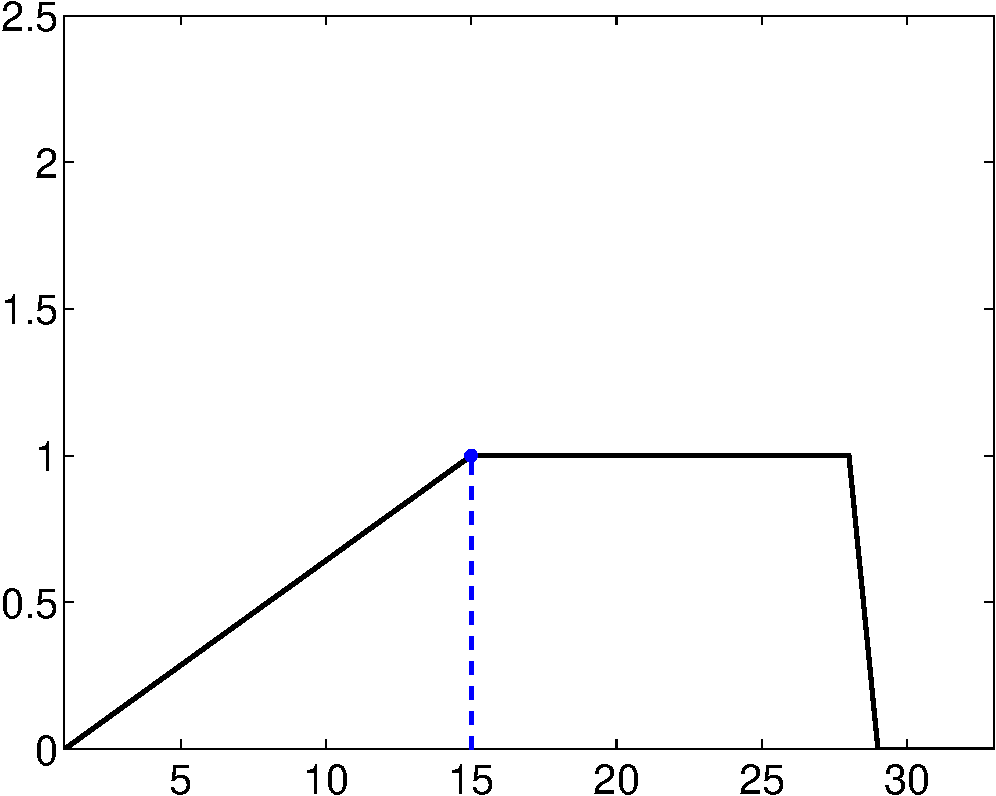
\includegraphics[width=0.425\textwidth]{./FigSparcoConvMask} &
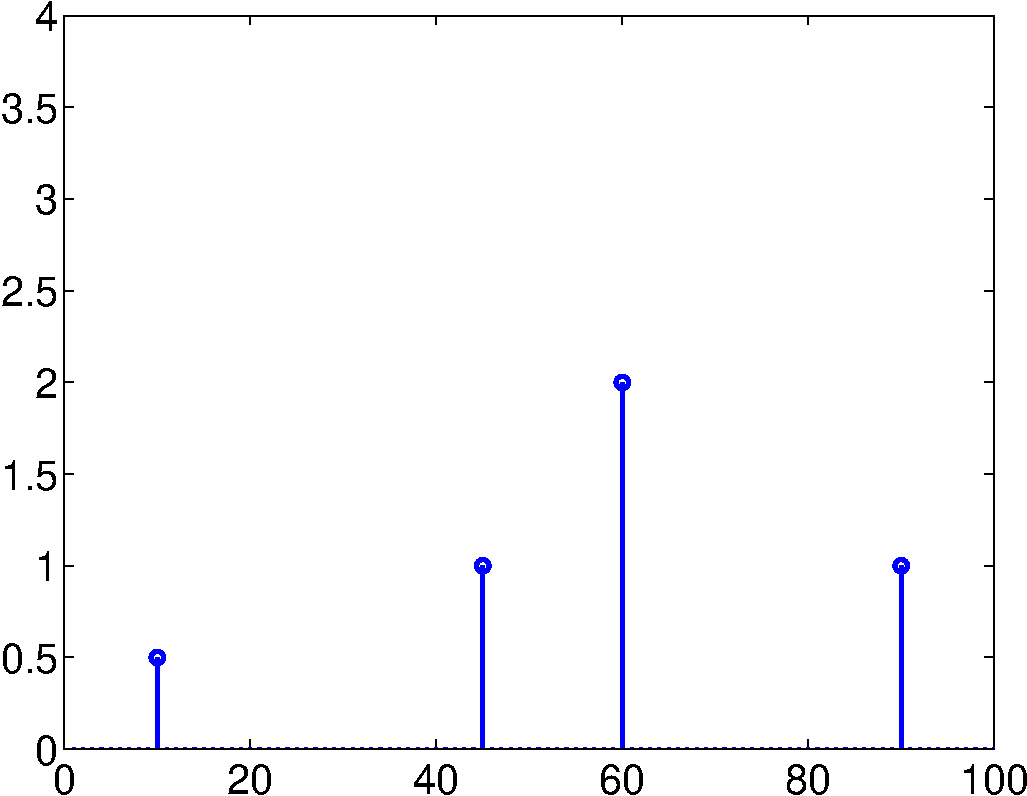
\includegraphics[width=0.425\textwidth]{./FigSparcoConvFun} \\
({\bf{a}}) & ({\bf{b}}) \\
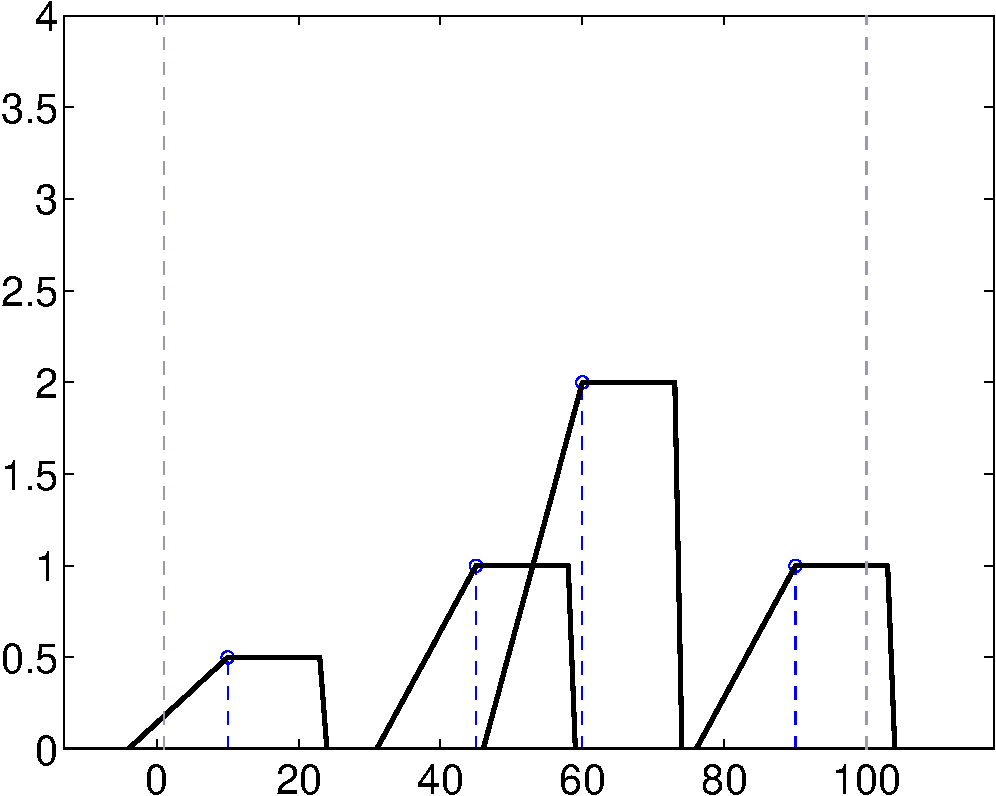
\includegraphics[width=0.425\textwidth]{./FigSparcoConvRegular1} &
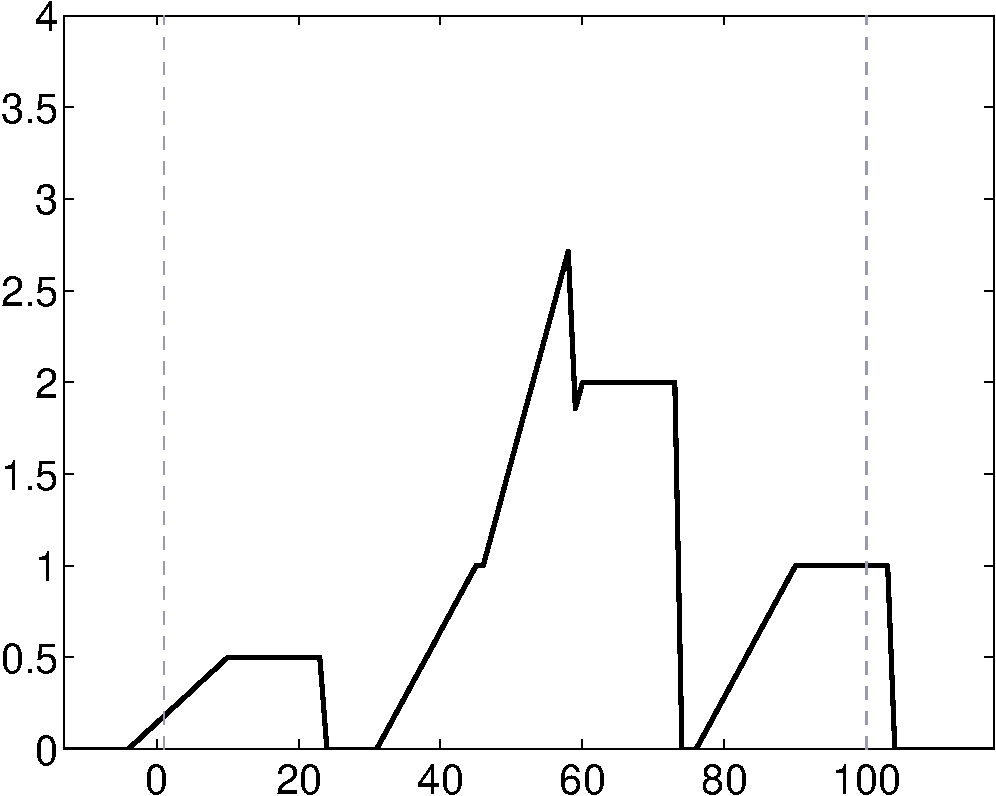
\includegraphics[width=0.425\textwidth]{./FigSparcoConvRegular2} \\
({\bf{c}}) & ({\bf{d}}) \\
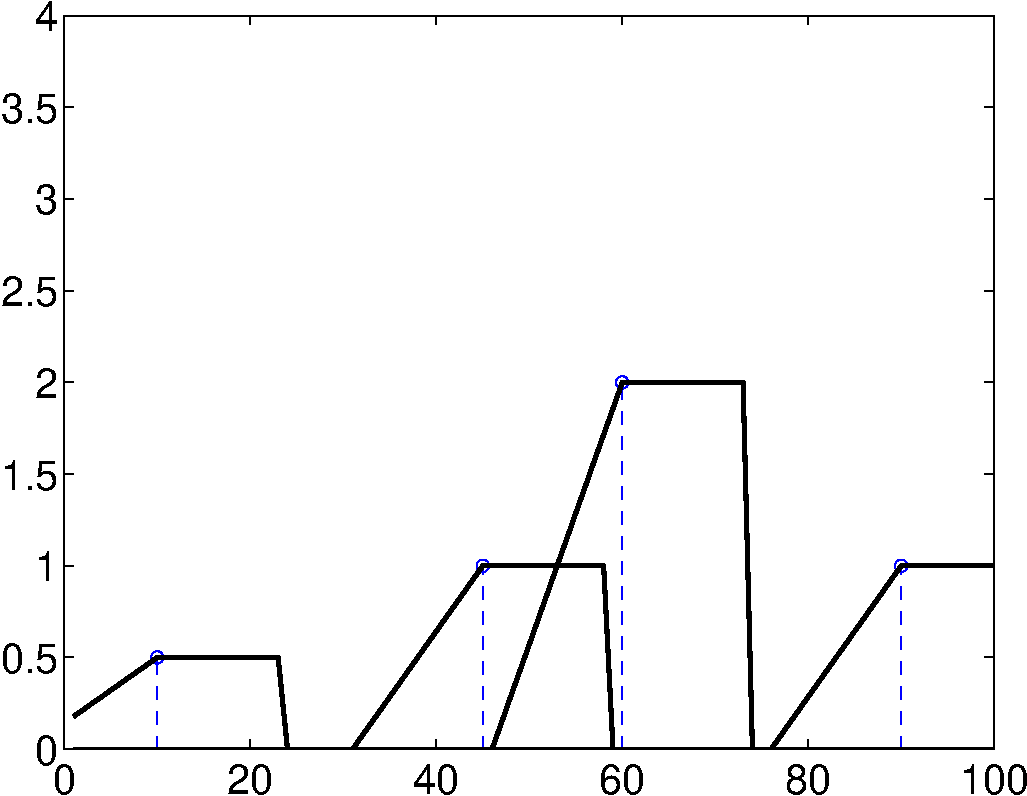
\includegraphics[width=0.425\textwidth]{./FigSparcoConvTrunc1} &
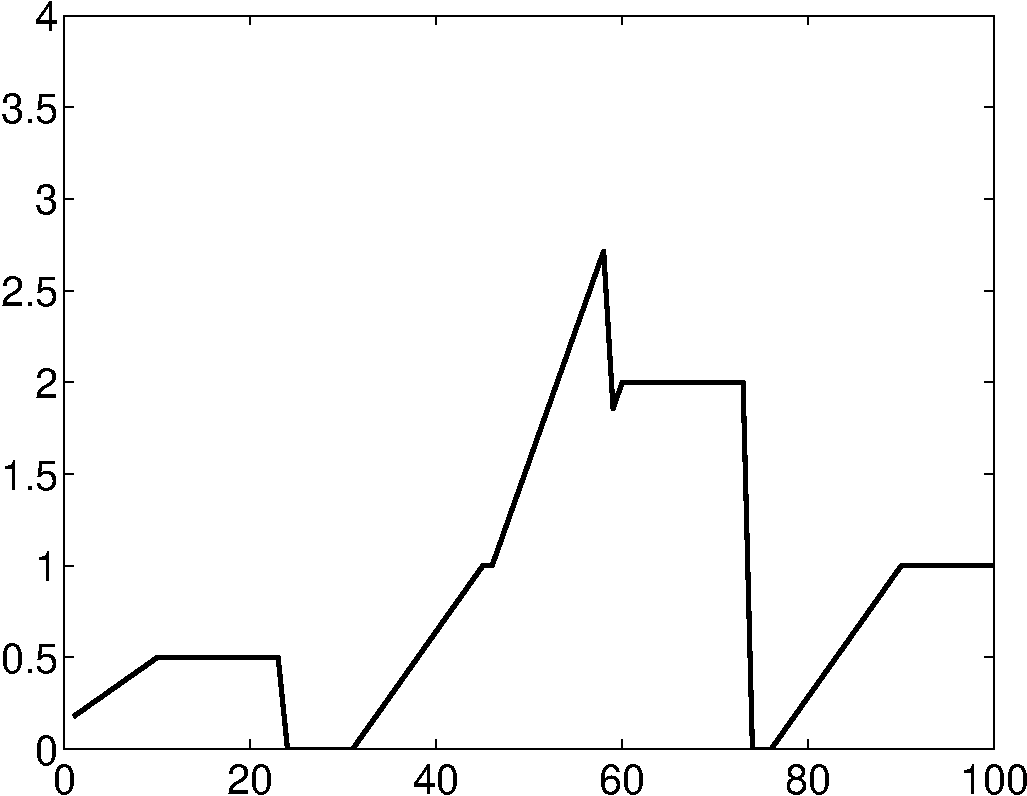
\includegraphics[width=0.425\textwidth]{./FigSparcoConvTrunc2} \\
({\bf{e}}) & ({\bf{f}}) \\
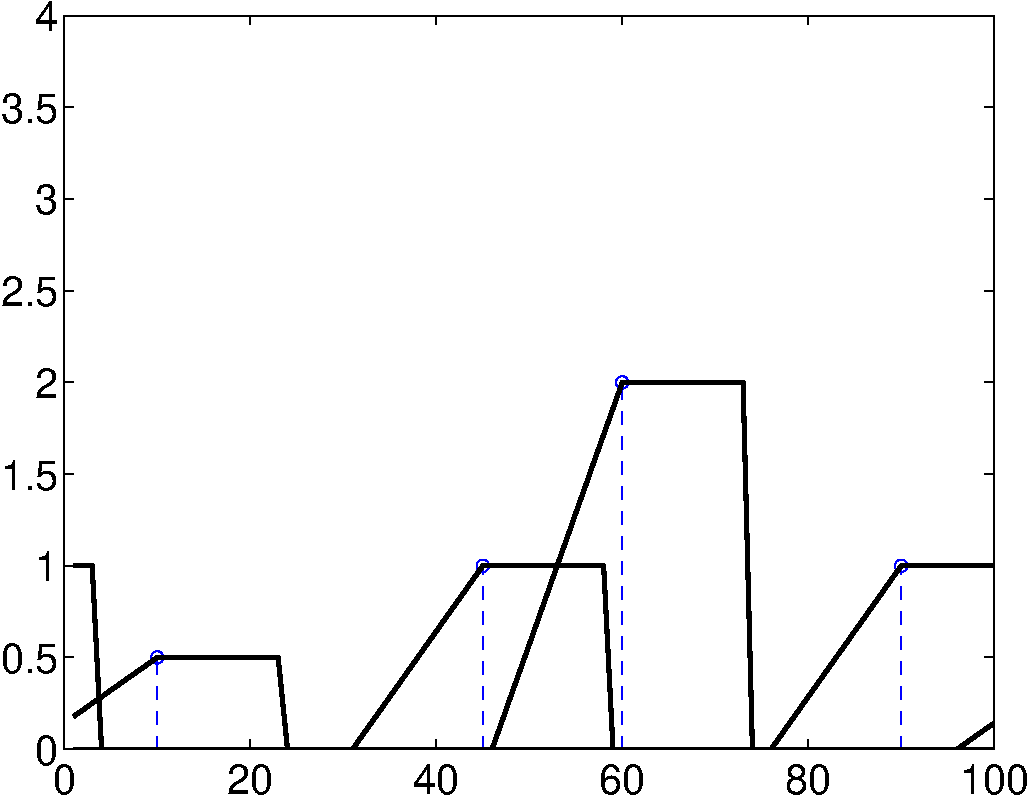
\includegraphics[width=0.425\textwidth]{./FigSparcoConvCycl1} &
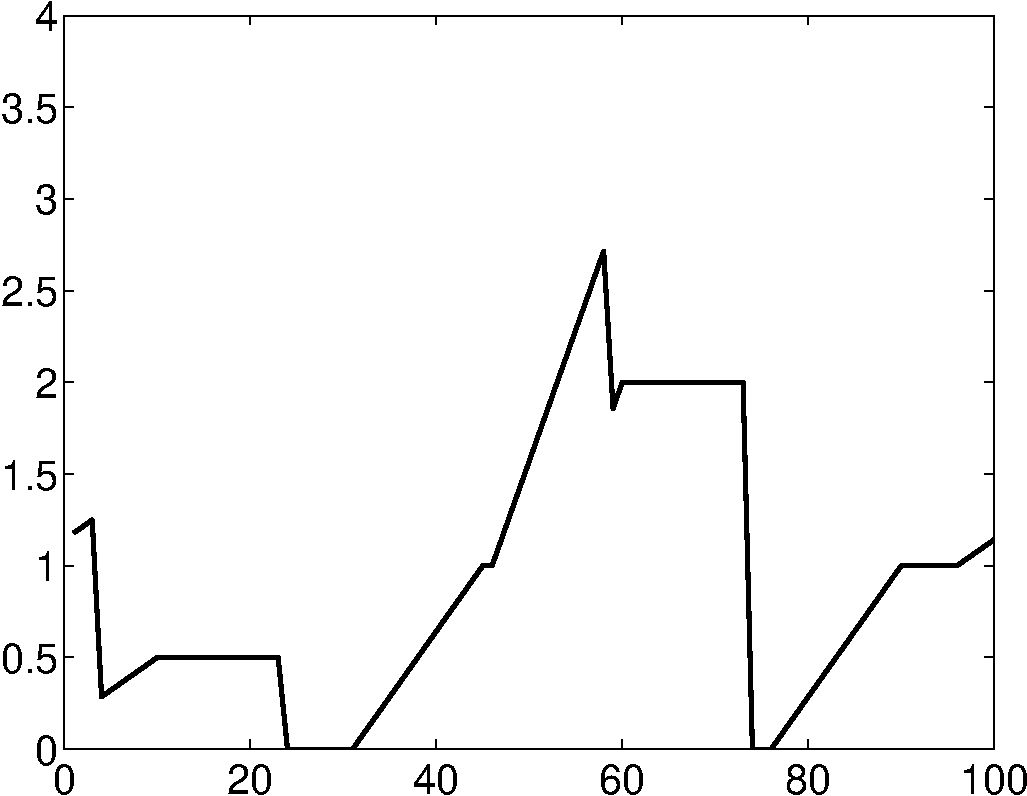
\includegraphics[width=0.425\textwidth]{./FigSparcoConvCycl2} \\
({\bf{g}}) & ({\bf{h}})
\end{tabular}
\caption{Illustration of the one-dimensional convolution operator; (a)
  convolution mask, (b) function, (c--d) regular convolution before
  and after summation, (e--f) truncated convolution, and (g--f) cyclic
  convolution.}\label{Fig:SparcoConvolution}
\end{figure}

%%% Local Variables: 
%%% mode: latex
%%% TeX-master: "manual"
%%% End: 

\chapter[Advanced issues]{Advanced issues and implementation details}
\label{Sec:SparcoImplementation}

The implementation of \spot{} is done using a mix of Matlab classes
and function handles. Each operator is a class that includes
information regarding its size, complexity, type, as well as a handle
to a function that applies the operator or its conjugate. Most users
will only be concerned with the (abstract) class interface described
in Chapter~\ref{Sec:SparcoMetaOp}, and the elementary operator
constructors described in Chapter~\ref{Sec:SparcoOperators}.  In this
chapter we look at more advanced issues and discuss certain aspects of
the implementation.

Readers familiar with object-oriented programming may wonder why
\spot{} has not been implemented using a class hierarchy in which each
operator is derived from some parent class. The main reason for this
is that in the current implementation, only a single new file needs to
be created anywhere, without prescribed directory naming conventions,
to define a new operator. This greatly simplifies the extension of
\spot{} and requires a minimum of knowledge about the implementation.

\section{Adding a new operator}

We discuss the addition of new operator based on the implementation of
the \mlcmd{opDCT} operator (simplified to one-dimensional transforms),
which provides a good example of the structure of a typical basic
operator. The implementation of meta-operators will be discussed
briefly in Section~\ref{Sec:SparcoNewMeta}.

\begin{codeblock}
function op = opDCT(n)
% OPDCT  One-dimensional discrete cosine transform (DCT)
%
%    More information about the operator.
%

fun = @(x,mode) opDCT_intrnl(x,mode);
op  = sparcoOp(fun,n,n,0,'DCT');

% Implementation of internal functions

function y = opDCT_intrnl(x,mode)
if mode == 1
   y = dct(full(x));
else
   y = idct(full(x));
end
\end{codeblock}

The first line of this code tells Matlab this is a function that takes
a single argument $n$ and outputs a variable called $op$. Following
the comment that is displayed when typing \mlcmd{help opDCT}, there
are two lines that construct the \spot{} operator. The first of the
two lines creates an anonymous function called \mlcmd{fun} that takes
two arguments: $x$, and $\mathrm{mode}$. Each time the \mlcmd{fun}
function is called Matlab invokes \mlcmd{opDCT\_intrnl} with the given
parameters. In this case we could equivalently have written \mlcmd{fun
  = @opDCT\_intrnl}, however, the above construction allows us to pass
additional (constant) parameters, such as matrix size, to the
underlying function. Once we have created a handle to a function op
two parameters that takes care of the operator application we can
instantiate the \spot{} class. This is done in the second of the two
lines:
\begin{codeblock}
op = sparcoOp(fun,n,n,0,'DCT');
\end{codeblock}
We discuss this function in more detail in Section
\ref{Sec:SparcoOpConstructor}.

The remainder of the example code consists of the implementation of
the operator itself. In most cases, these functions take two
parameters: an input vector of appropriate length, and a \mlcmd{mode}
that determines whether the operator ($\mathrm{mode} = 1$), or its
conjugate ($\mathrm{mode} = 2$) should be applied. Additional
parameters can be passed during the construction of the \mlcmd{fun}
function handle. In this case we simply check the \mlcmd{mode} and
call either \mlcmd{dct} or \mlcmd{idct} on the dense input vector, and
return the result, $y$.  In general, special care needs to be taken to
ensure that application to sparse or complex vectors, as well as
vectors containing NaN or Inf values is properly dealt with.


\section{The \mlcmd{sparcoOp} class}

Much of the administrative work, as well as the implementation of all
syntax overloading is done in the \mlcmd{sparcoOp} class. While the
exact details of the implementation are not important, its outside
interface is. This interface consists of the constructor function to
create new instances of the class, and the various ways in which
existing instances can be manipulated. We discuss both topics below.

\subsection{The \mlcmd{sparcoOp} constructor}
\label{Sec:SparcoOpConstructor}

The \mlcmd{sparcoOp} constructor takes a total of six arguments:
\begin{codeblock}
sparcoOp(op,m,n,cflag,type,data)
\end{codeblock}
Using the function handle, matrix, or \sparco{} operator given by
\mlcmd{op}, this creates an operator of size $m\times $n. In most
cases a handle to a function taking care of the application of the
operator on a vector is given. For meta-operators it is convenient to
convert all input arguments (including matrices and existing
operators) to \sparco{} operator using the constructor function,
without having to check their types. When \mlcmd{op} is a matrix it is
automatically converted to a \sparco{} operator using the
\mlcmd{opMatrix} command. Because the operator size is known for
matrices and operators, input arguments \mlcmd{m} and \mlcmd{n} are
ignored for these values of \mlcmd{op}. When one or both of the
dimensions of the operator is zero, \mlcmd{sparcoOp} returns an empty
operator of desired size.


The three remaining arguments provide more information about the
operator and are optional and used only in conjunction with function
handle input. The \mlcmd{cflag} is a logical scalar indicating whether
or not the operator is complex. When omitted, a real operator is
assumed. The \mlcmd{type} argument gives a string describing the type
of the operator. This information is used when printing information
about the operator, e.g., when using \mlcmd{disp}. It is highly
recommended to specify a type string because it is an empty string by
default. When specifying the type, make sure it does is not already
used for an existing operator, because this may cause trouble when
printing the operator (see \mlcmd{char.m} in the class directory when
in doubt). The last argument is a \mlcmd{data} structure that gives
additional information about the operator. A more detailed description
about predefined fields of this structure is given in Section
\ref{Sec:SparcoOp.data}.


\subsection{Attributes of the sparcoOp class}
\label{Sec:SparcoRealComplex}\label{Sec:SparcoOpFields}
\label{Sec:SparcoOpFieldLinear}\label{Sec:SparcoCounters}
\label{Sec:SparcoOp.data}

Attributes of class instances can be accessed either directly using
\mlcmd{op.field}, or using the \mlcmd{get} and \mlcmd{set}
functions. The following fields are defined

\begin{longtable}{|p{2.0cm}p{9.8cm}|}
\hline
\mlcmd{adjoint} & logic scalar that indicates whether the operator is
                  in adjoint mode or not \\
\mlcmd{linear}  & logic scalar that is set to true if the operator is
                  linear \\
\mlcmd{scalar}  & scalar multiplication factor associated with
                  operator \\ 
\mlcmd{counter} & a (possibly empty) string giving the name of a
                  variable in the base workspace that counts the
                  number of multiplications with the operator and its
                  adjoint \\
\mlcmd{type}    & a read-only string giving the type of the operator \\
\mlcmd{cflag}   & logic scalar that is set to true if the operator is
                  complex\\
\mlcmd{data}    & structure that contains additional, often
                  operator specific, information \\
\hline
\end{longtable}

\paragraph*{cflag} The \mlcmd{cflag} attribute indicates whether the
operator is complex or real. When combining operators, \spot{} has to
be conservative in deciding what value to use; it is not possible to
know in advance whether imaginary parts cancel out since each operator
is considered as a black box. This default behavior can be overridden
by the user by setting the \mlcmd{cflag}. Note that the \mlcmd{cflag}
attribute is concerned only with the complexity of the operator
itself, and not with the possible value of the \mlcmd{scalar}
field. For example, when we write \mlcmd{A = sqrt(-1) * opDCT(16)}, we
have \mlcmd{A.cflag = 0}, since $A$ is essentially the DCT
operator. Consequently, multiplying $A$ by some other purely imaginary
scalar yields a real operator. If we had updated the \mlcmd{cflag}
field, this information would have been lost. To query the complexity
of an operator it is recommended to use \mlcmd{isreal} function, which
does take the scalar quantity into account. The \mlcmd{clfag} is
mostly for internal use, but may be useful when developing a new
meta-operator.

\paragraph*{type} The \mlcmd{type} field is predominantly used when
displaying an operator. Besides this it is often used in the
development of self-aware meta-operators, as it allows them to check
if they apply a function to itself (for example, applying the complex
conjugate to itself will cancel the conjugation).

\paragraph*{counter} The \mlcmd{counter} field can be set to keep
track of the number of applications of the operator. This is done by
updating the associated variable in the base workspace. These counter
variables consist of two entries respectively counting the number of
direct and adjoint applications of the operator:
\begin{codeblock}
>> A = opMatrix(randn(3,4));
>> A.counter = 'aCounter';
>> A*randn(4,1); A*randn(4,1); A'*randn(3,1);
>> disp(aCounter)
     2     1
>> B = opBlockDiag(3,A);
>> B*randn(12,1);
>> disp(aCounter)
     5     1
\end{codeblock}
Note that writing \mlcmd{C = A'}, gives a new operator, which does
share the same counter as $A$. Multiplication by $C$ will be counted
as one multiplication by $A^H$ and vice versa though.

\paragraph*{adjoint} The \mlcmd{adjoint} attribute can be used to for
the complex transpose of the operator. Care has to be taken when
counters are associated with the operator whose \mlcmd{adjoint}
property is modified. Continuing from the above example:
\begin{codeblock}
>> disp(aCounter);
     5     1
>> A.adjoint = true;
>> A*randn(3,1);
>> disp(aCounter);
     5     2
\end{codeblock}
Although we multiply by $A$ itself (not its transpose), it is the
second entry of the counter variable that is updated. This is because
the counter variable was associated with the original $A$ and by
multiplying by the new $A$, we actually multiply by the transpose of
the original. We considered interchanging the counter entries upon
modifying the adjoint flag. However this may corrupt the counter when
writing \mlcmd{B = set(A,'adjoint',1)}, followed by multiplications
by $A$ (which still expects the original ordering).

\paragraph*{scalar} The \mlcmd{scalar} field provides a scalar
multiplier with which the operator is scaled. This scalar, when
complex, applies to the operator based on its present adjoint
state. When the adjoint state is changed by modifying the
\mlcmd{adjoint} property or by applying the complex transpose
operator, the scalar will automatically be changed to its complex
conjugate.

\paragraph*{Using the set command} When setting operator properties
using the \mlcmd{set} command, you must specify a left-hand side
variable:
\begin{codeblock}
A = set(A,'cflag',1)}
\end{codeblock}
otherwise the changes gets lost; a new variable is created which is
then immediately discarded. It is therefore usually easier to set the
fields directly using, e.g., \mlcmd{A.cflag = 1}, unless setting
multiple properties at once:
\begin{codeblock}
A = set(A,'linear',1,'cflag',0,'scalar',3)
\end{codeblock}
Finally, the \mlcmd{isfield} command can be used to check if a given
field is provided by the \mlcmd{sparcoOp} class.

\section{Adding a new meta-operator}\label{Sec:SparcoNewMeta}

Developing meta-operators is more complicated than regular operators,
and usually requires much more administrative code. In this section we
briefly discuss a number of things that need to be kept in mind when
developing a new meta-operator.

The first thing to do when writing a constructor function for a
meta-operator is to check the input arguments, and convert all
matrices to operators using the \mlcmd{sparcoOp}
function. Compatibility of the operators then needs to be checked, and
the complexity and linearity of the resulting operator determined. The
next step then, like that of basic operators, is to create a handle to
a function implementing multiplication by the meta-operator and its
complex transpose.

By their very nature meta-operators always need to maintain a list of
operators they depend on. This list is easily passed to the
multiplication function in the definition of the anonymous function:
\begin{codeblock}
fun = @(x,mode) intrnl\_fun(oplist,x,mode);
\end{codeblock}
This list is also required when displaying the operator and for
cell-indexing (see Section \ref{Sec:CellIndexing}). To facilitate
this, the \mlcmd{data} structure has a reserved field called
\mlcmd{oplist}, which should be set prior to calling \mlcmd{sparcoOp}
to complete the operator:
\begin{codeblock}
data = struct();
data.oplist = oplist;
fun         = @(x,mode) ...;
op          = sparcoOp(fun,m,n,cflag,name,data);
\end{codeblock}
Other attributes, such as the linearity should be set after the
operator is created.

When certain meta-operators, such as \mlcmd{opConj} and
\mlcmd{opInverse}, are applied to themselves they can often be
simplified. When doing such simplifications it is important to check
the \mlcmd{adjoint} and \mlcmd{scalar} fields. For example, when
unpacking a conjugate operator, any scalar multiplier associated with
the outer operator has to be conjugated and multiplied by the original
scalar. When manipulating the scalars, it is best to do this by
setting the \mlcmd{scalar} field directly. This avoid accidental
multiplication by scalar vector resulting an a numeric vector rather
than a new operator.


\section{Cell indexing}\label{Sec:CellIndexing}

In \spot{} the cell-indexing operation is overloaded to provide
(read-only) access to the operators that make up a given
operator. This is best illustrated by a simple example. Assume we have
the following definitions:
\begin{codeblock}
A = opEye(8);
B = opFFT(8);
C = opGaussian(8,16);
D = [A,B];
E = C + D;
F = C + D + 2;
\end{codeblock}
Then
\begin{codeblock}
>> D{2}
ans is a linear Sparco operator of size 8 x 8
         FFT(8,8)
>> E{1}
ans is a linear Sparco operator of size 8 x 16
         Gaussian(8,16)
>> E{2,1}
ans is a linear Sparco operator of size 8 x 8
         Eye(8,8)
>> data = F{2:3}
data =
    [8x16 sparcoOp]    [8x16 sparcoOp]
\end{codeblock}
By combining cell indexing with property access it is possible to
obtain the properties of a range of sub-operators:
\begin{codeblock}
>> F{:}.cflag
ans =
    [0]    [1]    [0]
>> F{2}.data
ans =
    oplist: {[8x8 sparcoOp]  [8x8 sparcoOp]}
>> F{2}.data.oplist{1}
ans is a linear Sparco operator of size 8 x 8
         Eye(8,8)
\end{codeblock}
As mentioned above, cell indexing is read-only, and intended only to
get information. It is not possible to modify or set properties of
underlying operators.

Operations such as \mlcmd{opFoG}, \mlcmd{opSum}, and
\mlcmd{opDictionary} do not check whether their arguments are of the
same type (in that case they could be unwrapped and added to the
operator list). This is done mostly to keep operators as a unit.
Consider the following example:
\begin{codeblock}
C = A * B;
E = C * A
\end{codeblock}
In this case we would like \mlcmd{E} to consist of two operator,
instead of three which would be the case when expanding \mlcmd{C} to
give \mlcmd{E = A*B*D}.  This does bring with it a slight
problem. When matlab sees \mlcmd{A*B*D} it will call the \spot{}
multiplication operator first on \mlcmd{A*B} and then multiply that
the result by \mlcmd{D}, giving \mlcmd{(A*B)*D}. Setting \mlcmd{E =
  A*B*D} would then consist of two operators: \mlcmd{(A*B)} and
\mlcmd{D}, which is unnatural. To overcome this situation and make it
more intuitive \spot{} checks whether the operators it sees are
named. If they are not named we can assume they are intermediate
results and expansion is done. This means that \mlcmd{E = A*B*D} does
consist of three operators. This remains so even when \mlcmd{B} is
itself a product of operators. The same applies to addition and
subtraction. In dictionaries, \spot{} gets all elements at once so no
effort is required here. Scalar multiplication is included in the
appropriate operator:
\begin{codeblock}
>> X = A + A + 3*(A+A);
>> X{3}
ans is a linear Sparco operator of size 8 x 8
         3 * (Eye(8,8) + Eye(8,8))
\end{codeblock}

\section{Known issues}

\paragraph{Cell indexing} When using cell indexing on a compound
operator to get its constituent operators, it is not possible to use
\mlcmd{end} to get the last operator. The reason for this is that,
when seeing the \mlcmd{end} keyword, \matlab{} calls the \mlcmd{end}
function implemented by the operator to get the corresponding
number. Unfortunately, it does not specify whether \mlcmd{end} was
used within array indexing \mlcmd{[]} or within cell indexing
\mlcmd{\{\}}. It was therefore decided to always return the desired
dimension of the operator rather than the number of operators used to
create it. This will lead to somewhat unexpected results when using
the \mlcmd{end} keyword within cell indexing.

\paragraph{Scalar multiplication} When post-multiplying an $n\times 1$
\sparco{} operator by a scalar this will be interpreted as a
matrix-vector operation giving a numeric result, rather than a scaled
version of the operator (which is generally the case). This follows
from the rule that multiplication between an operator and an
appropriately sized matrix or vector leads to the evaluation of the
product. Scalar multiplication is considered only after this rule has
been applied. The reason behind this choice in priority is that the
conversion of an operator to an array, \mlcmd{double(op)}, would
otherwise not work properly for $n\times 1$ operators. A similar
situation arises when pre-multiplying a $1\times n$ operator by a
scalar. When scalar multiplication of such operators is needed you can
either pre-, respectively post-multiply by a scalar, thereby avoiding
evaluation, or directly set the \mlcmd{.scalar} property op the
operator.

%%% Local Variables: 
%%% mode: latex
%%% TeX-master: "manual"
%%% End: 


\chapter*{Acknowledgements}
\addcontentsline{toc}{chapter}{Acknowledgements}

Many thanks to Gilles Hennenfent, Felix Herrmann, Evgeniy Lebed, Rayan
Saab, and \"{O}zgur Y{\i{}}lmaz for their contributions and support
during the development of \spot{}. We would also like to thank Igor
Carron for promoting the use of the compressed sensing problem suite
\sparco{} which led to the development of \spot{}. A final thanks to
Rice digital signal processing (DSP) group for making available their
wavelet toolbox for distribution with \spot{}.


\appendix
\chapter{Window functions}\label{Sec:SparcoWindowFunc}

% Parzen window unclear, scale discrete mesh from -1 to 1?

% On the use of windows for harmonic analysis with the discrete Fourier transform
% Harris, F.J.  
% This paper appears in: Proceedings of the IEEE
% Publication Date: Jan. 1978
% Volume: 66,  Issue: 1
% On page(s): 51- 83
% ISSN: 0018-9219
% Date Published in Issue: 2005-06-28 14:49:59.0
% Abstract: This paper makes available a concise review of data
% windows and their affect on the detection of harmonic signals in the
% presence of broad-band noise, and in the presence of nearby strong
% harmonic interference. We also call attention to a number of common
% errors in the application of windows when used with the fast Fourier
% transform. This paper includes a comprehensive catalog of data
% windows along with their significant performance parameters from
% which the different windows can be compared. Finally, an example
% demonstrates the use and value of windows to resolve closely spaced
% harmonic signals characterized by large differences in amplitude.

% N is number of samples, n  http://en.wikipedia.org/wiki/Window_function

Define $k:= \left\vert \frac{2n}{N-1} - 1\right\vert$, for
$n=0,\ldots,N-1$, as the normalized offset from the center; i.e.,
corresponding to the samples $0 \leq \vert \ell\vert \leq
\frac{N}{2}$, normalized to the range $0$ to $1$.

\begin{longtable}{|p{3.1cm}p{10cm}|}
\hline
Bartlett & 
      $\displaystyle w(k) = 1 - k$ \\
&\\ Bartlett-Hann &
   $\displaystyle w(n) = a_0 -
   a_1\left\vert \frac{n}{N-1}- \frac{1}{2}\right\vert -
   a_2\cos\left(\frac{2\pi n}{N-1}\right)$ \\ 
  & \footnotesize with $a_0 = 0.62$, $a_1 = 0.48$, $a_2 = 0.38$ \\
&\\ Blackman &
   $\displaystyle w_{\alpha}(n) = \sum_{j=0}^2 a_j(-1)^j \cos\left(\frac{2j\pi
   n}{N-1}\right)$ \\
  & \footnotesize with $a_0 = (1-\alpha)/2$, $a_1 = 1/2$, $a_2 = \alpha / 2$ \\
&\\ Blackman-Harris &
   $\displaystyle w(n) = \sum_{j=0}^3 a_j(-1)^j \cos\left(\frac{2j\pi
   n}{N-1}\right)$ \\
  & \footnotesize with $a_0 = 0.35875$, $a_1 = 0.48829$, $a_2 = 0.14128$, $a_3 = 0.01168$ \\
&\\ Blackman-Nuttall &
   $\displaystyle w(n) = \sum_{j=0}^3 a_j(-1)^j \cos\left(\frac{2j\pi
   n}{N-1}\right)$ \\
  & \footnotesize with $a_0 = 0.3635819$, $a_1 = 0.4891775$,
   $a_2 = 0.1365995$, $a_3 = 0.0106411$ \\
&\\ Bohman &
   $\displaystyle w(k) = (1 - k)
   \cos(\pi k) +
   \frac{1}{\pi}\sin(\pi k) $ \\
&\\ Cauchy &
   $\displaystyle w_{\alpha}(k) = \frac{1}{1 + (\alpha\cdot k)^2}$ \\
&\\ Cos & See cosine \\
&\\ Cosine &
   $\displaystyle w_{\alpha}(k) = cos^{\alpha}\left(\frac{k\pi}{2}\right)$ \\
&\\ Dirichlet & 
   $\displaystyle w(k) = 1$ \\
&\\ Flat top / Flattop&
   $\displaystyle w_{\alpha}(n) = \textstyle\frac{1}{\sum_{j=0}^4 a_i}
   \displaystyle \sum_{j=0}^4 a_j(-1)^j \cos\left(\frac{2j\pi
   n}{N-1}\right)$ \\
  & \footnotesize with $a_0 = 1$, $a_1 = 1.93$, $a_2 = 1.29$, $a_3 =
  0.388$, $a_4 = 0.032$ \\
&\\ Gauss & See Gaussian \\
&\\ Gaussian & 
  $\displaystyle w_{\alpha}(k) =
  \mathrm{exp}\left(-\frac{1}{2}\left(\alpha k\right)^2\right)$\\
&\\ Hamming &
   $\displaystyle w(n) = a_0 - a_1\cos\left(\frac{2\pi
   n}{N-1}\right)$  \\
   & \footnotesize with $a_0 = 0.54$, $a_1 = 0.46$ \\
&\\ Hann &
  $\displaystyle w(n) = \frac{1}{2}\left(1 - \cos\left(\frac{2\pi
  n}{N-1}\right)\right)$ \\
&\\ Hann-Poisson &
  $\displaystyle w_{\alpha}(k) = \frac{1}{2}\left[1 + \cos\left(\pi k)\right]\right)\exp\left(-ak\right)$ \\
&\\ Kaiser &
   $\displaystyle w_{\alpha}(k) = I_0\left(\alpha\sqrt{1 -
   k^2}\right)/I_0(\alpha)$  \\
   & \footnotesize with $I_0$ the zeroth-order modified Bessel
   function of the first kind \\
&\\ Kaiser-Bessel\ \ \ \ \ \ \ \ \ Derived (KBD) & 
   $\displaystyle w_{\alpha}(n) = \begin{cases} 
   c\left(\sum_{j=0}^n v_{\alpha}(j)\right)^{1/2},
   & \ \ 0 \leq n < N/2 \\
   c\left(\sum_{j=0}^{N-n-1} v_{\alpha}(j)\right)^{1/2},
   
   & \ \ N/2 \leq n < N
 \end{cases}$ \\
 & \footnotesize with $c=\left(\sum_{j=0}^{N/2}
   v_{\alpha}(j)\right)^{-1/2}$, $v_{\alpha}(n)$ the $(N/2+1)$-point
 Kaiser
 window. $N$ must be an even number.\\
   % http://ccrma.stanford.edu/courses/422/projects/kbd/kbdwindow.cpp
   % http://en.wikipedia.org/wiki/Kaiser_window
&\\ Lanczos &
   $\displaystyle w_{\alpha}(k) = \left(\frac{\sin(\pi k)}{\pi k}\right)^{\alpha}$ \\
&\\ Nuttall &
   $\displaystyle w(n) = \sum_{j=0}^3 a_j(-1)^j \cos\left(\frac{2j\pi
   n}{N-1}\right)$ \\
  & \footnotesize with $a_0 = 0.355768$, $a_1 = 0.487396$,
   $a_2 = 0.144232$, $a_3 = 0.012604$ \\
&\\ Parzen & 
   $\displaystyle w(t) = \begin{cases}
   1 - 6\left(\frac{t}{N/2}\right)^2\left(1 - \frac{\vert
       t\vert}{N/2}\right), & \ \ 0 \leq \vert t\vert \leq \frac{N}{4} \\
   2\left(1 - \frac{\vert t\vert}{N/2}\right)^3, &
   \ \ \frac{N}{4} \leq \vert t\vert \leq \frac{N}{2}   
   \end{cases}$ \\
% Mathematical Considerations in the Estimation of Spectra
% Emanuel Parzen
% Technometrics, Vol. 3, No. 2 (May, 1961), pp. 167-190 
&\\ Poisson & See Lanczos, $\alpha = 1$
   $\displaystyle w(k) = \exp\left(-ak\right)$ \\
&\\ Rectangle & See Dirichlet \\
&\\ Riesz &
   $\displaystyle w(k) = 1 - \vert k\vert^2$ \\
&\\ Sinc & See Lanczos \\
&\\ Triangle & 
   $\displaystyle w(k) = 1 - k$\\
&\\ Tukey & 
   $\displaystyle w_{\alpha}(t) = \begin{cases}
   1, & 0 \leq \vert t\vert \leq \alpha\frac{N}{2} \\
   \displaystyle\frac{1}{2} + \frac{1}{2}\cos\left(\frac{\pi}{2}\cdot
   \frac{2t/N - \alpha}{1 - \alpha}\right), &
   \alpha\frac{N}{2} \leq \vert
   t\vert \leq \frac{N}{2}
   \end{cases}$ \\
&\\ Uniform & See Dirichlet \\
&\\ Vall\'e-Poussin & See Parzen \\
&\\ Weierstrass & See Gaussian \\
\hline
\end{longtable}

%%% Local Variables: 
%%% mode: latex
%%% TeX-master: "manual"
%%% End: 

\chapter{Dependencies}

\begin{longtable}{|p{2.4cm}p{9.4cm}|}
\hline
\mlcmd{opWavelet}
& Rice wavelet toolbox \cite{RWT}, included in distribution \\
\mlcmd{opHaar1d}
& Rice wavelet toolbox \cite{RWT}, included in distribution \\
\mlcmd{opHaar2d}
& Rice wavelet toolbox \cite{RWT}, included in distribution \\
\mlcmd{opCurvelet2d}
& CurveLab 2.0 \cite{Curvelet}, not included \\
\mlcmd{opSurfacelet}
& Surfacelet Toolbox \cite{SurfaceletToolbox}, not included \\
\mlcmd{opDCT}
& \mlcmd{sparcoDCT.m}, \mlcmd{sparcoIDCT}.m, included \\
\mlcmd{opInverse}
& \mlcmd{sparcoLSQR.m}, by Paige and Saunders \cite{PaigSaun:1982},
included \\ 
\hline
\end{longtable}

%%% Local Variables: 
%%% mode: latex
%%% TeX-master: "manual"
%%% End: 


\bibliography{sparco}
\addcontentsline{toc}{chapter}{Bibliography}


\end{document}